\documentclass[10pt,letterpaper]{article}
\usepackage[left=1.8cm, right=1.8cm, top=1cm]{geometry}
\usepackage[utf8]{inputenc}
\usepackage[T1]{fontenc}
\usepackage[spanish]{babel}
\usepackage{amsmath}
\usepackage{amsfonts}
\usepackage{amssymb}
\usepackage{graphicx}
\usepackage{subfigure}
\usepackage{steinmetz}
\usepackage{float}
%\usepackage{circuitikz}

\author{Clase Práctica $\#$7}
\title{Electrónica I}
\date{Diodos.}

\renewcommand{\sin}{\sen}
\begin{document}
	\maketitle
	
Bibliografía: Electrónica: Teoría de Circuitos y Dispositivos Electrónicos. Robert L. Boylestad y Louis Nashelsky, 10ma ed. Capítulo 1.
\\

1- Calcular la tensión y la corriente en la resistencia de $1 \: \mathrm{k}\Omega$ y la potencia en el diodo en la siguiente figura empleando:

a) la aproximación del diodo ideal.

b) la segunda aproximación o modelo simplificado.

c) la tercera aproximación o modelo lineal por segmentos, considerando una resistencia interna de $23 \: \Omega$.

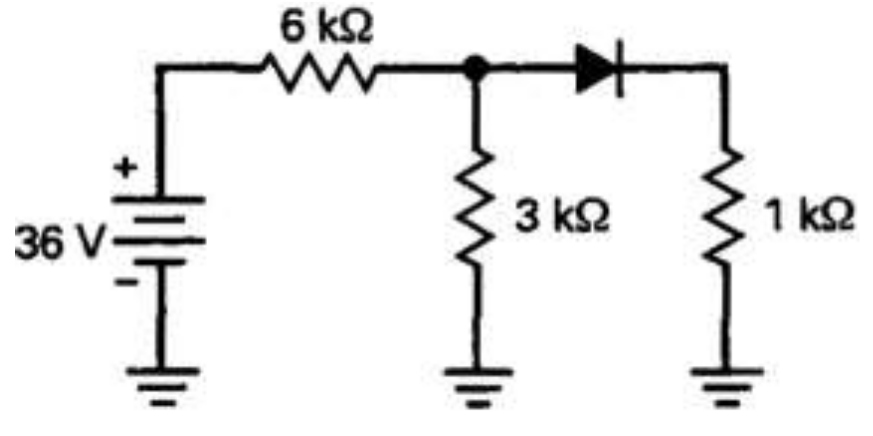
\includegraphics[scale=0.27]{c1.png} 
\\

%2-Calcule la caída de tensión y la corriente que fluye en el diodo del circuito de la figura. Considere conocidos los valores de I, V, $\mathrm{R_1}$, $\mathrm{R_1}$, $\mathrm{R_1}$ y la curva I-V del diodo.
%
%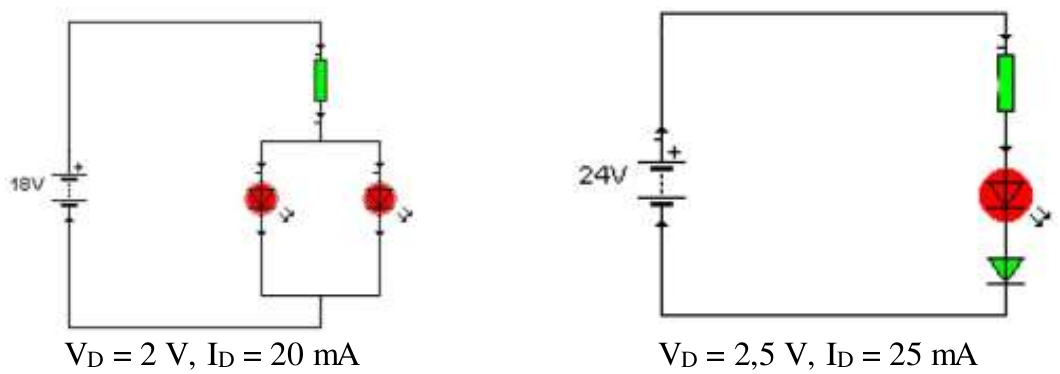
\includegraphics[scale=0.27]{c2.png} 

2- Hallar en cada caso (a y b) el valor de la resistencia para que el LED no se queme y funcione con los valores indicados.

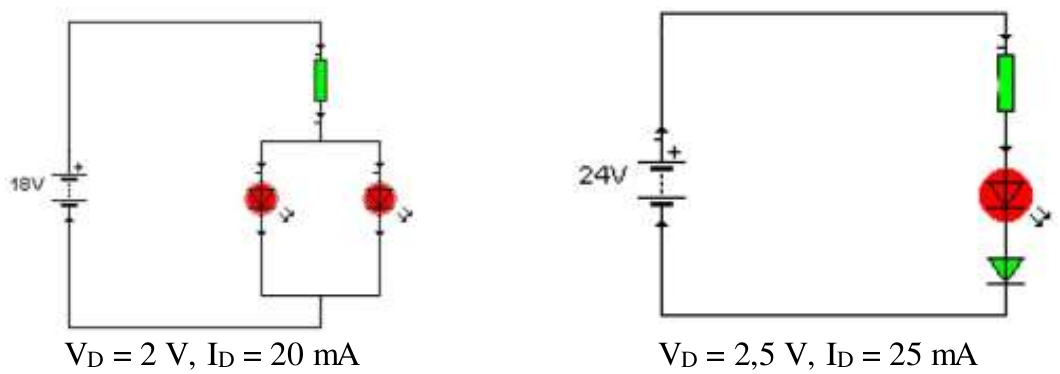
\includegraphics[scale=0.35]{c2.png} \\

3- Trace la forma de onda de $i$ de la red de la figura si $t_t = 2t_s$ y el tiempo de recuperación en inversa es de $9 \: \mathrm{ns}$.

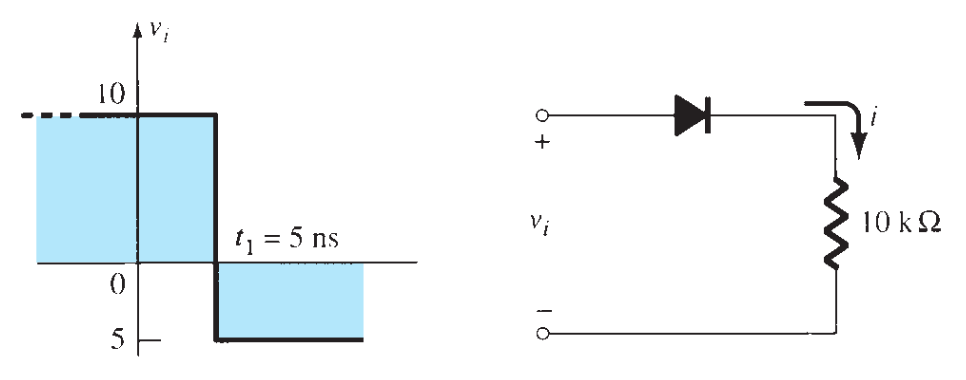
\includegraphics[scale=0.35]{c3.png} 

4- Calcular la potencia mínima del diodo zener de la figura, para que el circuito estabilice correctamente, si la entrada del circuito puede variar entre 10 y 15 V y $\mathrm{R_L}$ entre 1 y 10 $\: \mathrm{k}\Omega$ El diodo zener tiene una tensión zener de 5 V y la resistencia R del circuito un valor de 100 $\Omega$. \\

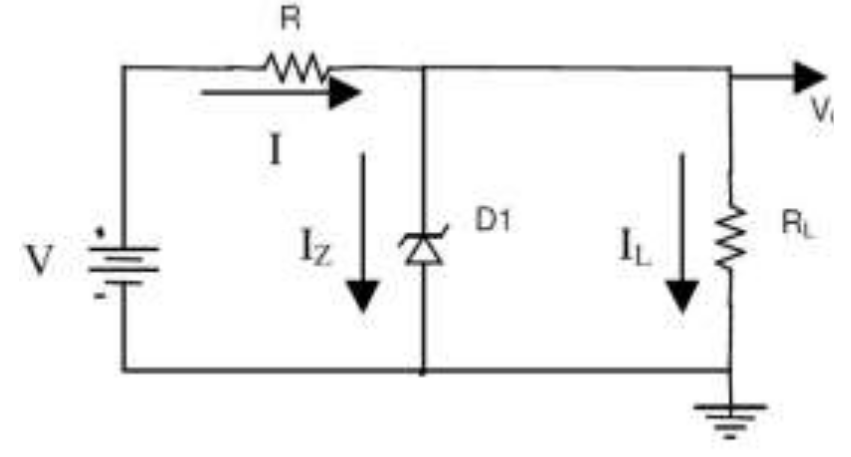
\includegraphics[scale=0.35]{c4.png}

5- Determine la reactancia ofrecida por un diodo descrito por las características de la figura, con un potencial en directa de 0.2 V y un potencial en inversa de 20 V si la frecuencia aplicada es de 6 MHz. 

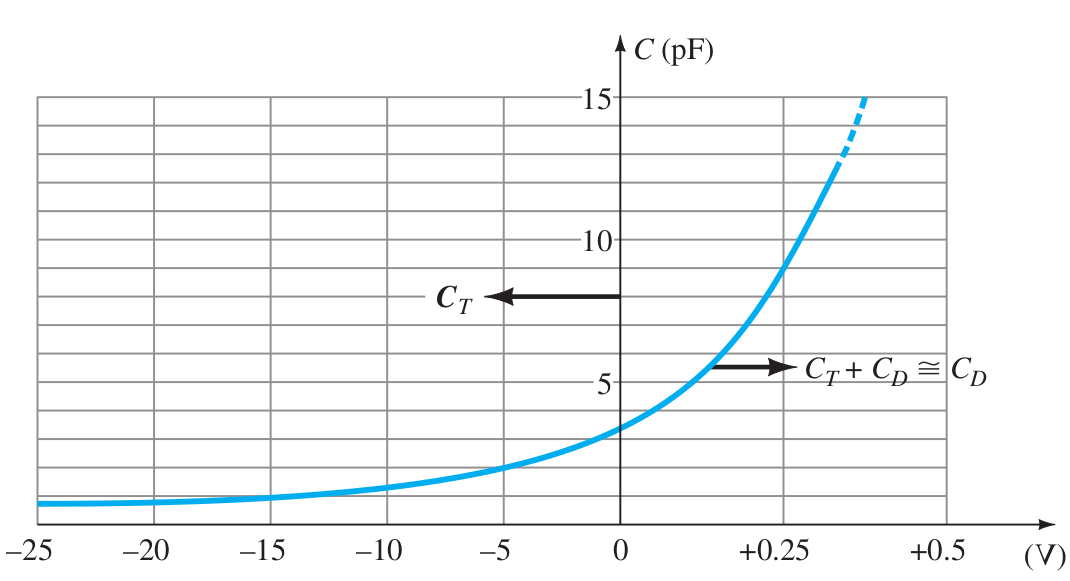
\includegraphics[scale=0.35]{c5.png}

\end{document}